\section{Mission Description}
\label{sec:mission}
An inspector spacecraft with induction couplers can fulfill a number of functions including verifying the state of health, performing mechanical tasks, or providing communications and other logistical support for astronauts during extravehicular activity (EVA). It may be possible for the eddy currents use for locomotion to detect mechanical damage, as is currently done on some aircraft. \cite{Yang2010}
 This paper focuses on the International Space Station (ISS), but a similar inspection spacecraft could enable unique OOS missions to inspect and repair other large satellites.

The inspection spacecraft described here uses induction couplers to pull itself along the aluminum exterior of the ISS, maintaining a separation distance of a few centimeters. In doing so, it acts like a damage-inspection Roomba,\cite{Tribelhorn2007}
 canvassing the surface and automatically detecting damage from micrometeorite strikes. An alternative operations concept is one in which the inspector is controlled directly by an astronaut to evaluate some region of interest and possibly use an attached robotic arm to effect a repair. In yet another concept, the spacecraft acts like an extra pair of hands during an EVA, remaining near an astronaut and holding tools. NASA's Robonaut and the Mobile Servicing System (the Canadian robotic arm on ISS) have demonstrated the value of such a capability but are limited by rails to specific locations. \cite{Ambrose2012}
The ability to traverse the exterior of the ISS without being constrained to travel on rails, attach to specific hard points, or manage a finite propellant supply can free up one of the most valuable resources on the ISS, astronaut time, and may augment astronaut safety.

\begin{figure}
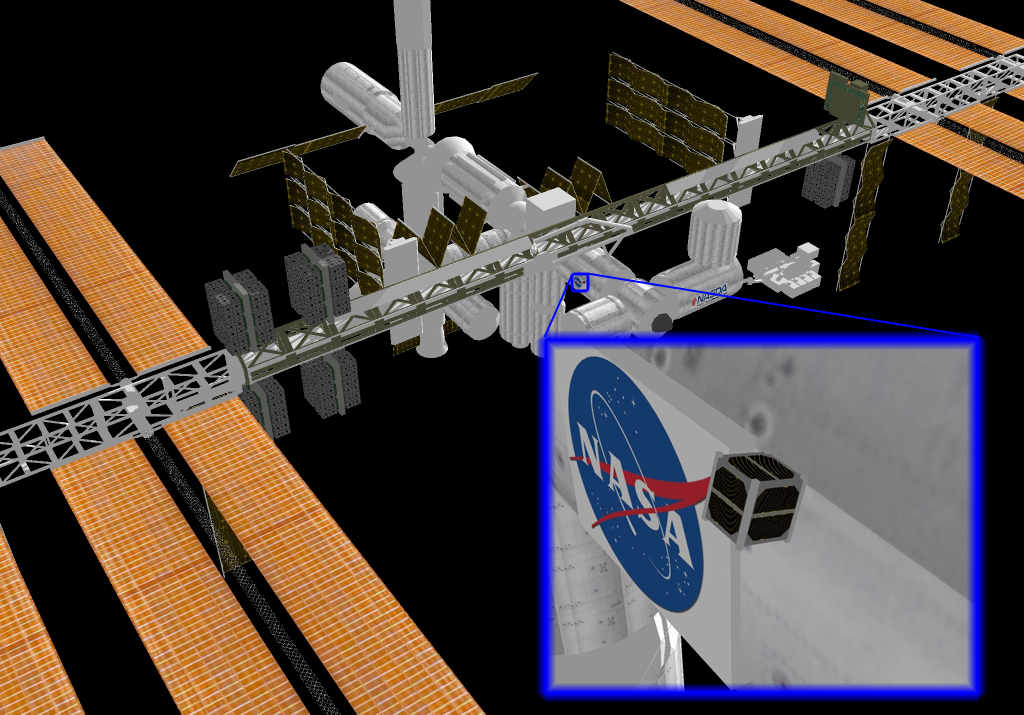
\includegraphics[width = 6cm, height = 6cm ]{figures/iss_inspector.jpg}
\caption{A chaser traverses the surface of the ISS using induction couplers}
\label{fig:iss_inspector}
\end{figure}